\documentclass{article}
\usepackage{graphicx}
\usepackage{amsmath}
\usepackage{hyperref}
\title{Sin(x) }
\author{Villads Jacobsen}

\begin{document}
\maketitle

This paper will examine the trigonometric function sin(x) and the numerical integral of such function.
The sin(x) is given as the sum of:


\begin{equation}
sin(x)=\sum_n^{\infty} =\frac{(-1)^n}{(2n+1)!}x^{2n+1}
\end{equation}

and is closely related to cos(x) and tan(x) in the field of trigonometry, where they are used to
calculate sides and angles of different triangles. Sin(x) also relates to cos(x) through differentiation and integration.

\begin{itemize}
 \item sin(x)' = cos(x) 
 \item cos(x)' = -sin(x)
\end{itemize}

Which leads to the fact that sin(x) anti derrivative is -cos(x). In figure \cite{fig:sinusintegral} we have the integral of
sin(x) from 0 to 2 pi. If -cos(x) is the anti-derivative then the integral from 0 to pi should be 2 (cos(0)-cos(pi)=2). We se from the figure that
the peak value at pi is in fact 2, so the numerical integrator agrees with the analytical result.


\begin{figure}
\caption{This shows the integral of sin(x) from 0 to 2 pi}
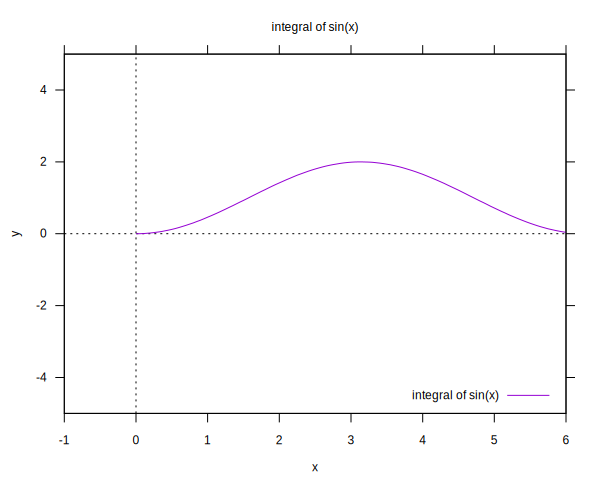
\includegraphics[width=\columnwidth]{plot.png}
\label{fig:sinusintegral}
\end{figure}




\end{document}
